\documentclass[11pt]{article}

\usepackage[a4paper,margin=1in]{geometry}
\usepackage{amsmath,amssymb}
\usepackage{booktabs}
\usepackage{graphicx}
\usepackage{hyperref}
\usepackage{siunitx}
\usepackage{subcaption}
\usepackage{float}

\hypersetup{
  colorlinks=true,
  linkcolor=blue,
  urlcolor=blue,
  citecolor=blue
}

\newcommand{\GL}{\textsc{GammaLoop}}
\newcommand{\dd}{\mathrm{d}}
\newcommand{\abs}[1]{\left|#1\right|}

\title{Double-UV Relative-Momentum Enhancement in the GL00 \texorpdfstring{$\gamma\gamma\to\gamma\gamma$}{aa to aa} Integrand}
\author{Investigation note}
\date{\today}

\begin{document}
\maketitle

\begin{abstract}
This note documents the current understanding of a large-weight feature seen in
the generated GL00 two-loop integrand for
$\gamma\gamma\to\gamma\gamma$ with the nested integrated UV counterterm
included.  The issue is not an ordinary uncancelled UV divergence in a generic
double-UV direction.  The problematic samples lie close to a relative-momentum
ridge: two sampled loop-momentum-basis (LMB) rays become hard, nearly collinear,
and have comparable radii, so that one physical internal momentum is a small
difference of the two hard basis momenta.  The resulting enhancement is locally
integrable, but it creates large Monte-Carlo variance because the current
sampling channels do not parameterize that relative momentum directly.  LMB
multichanneling is not merely a random choice of LMB: it includes a normalized
OSE-product prefactor, and that prefactor strongly suppresses inappropriate
channels near the edge-small limit.  The remaining question is how much this
discrete reweighting, and in particular its exponent $\alpha$, can reduce the
variance without an additional continuous relative-momentum map.  A fixed-ray
option was added to the UV profiler to make this non-generic direction visible
in profiling runs.
\end{abstract}

\section{Executive summary}

For the regenerated all-LMB setup, \GL{} reports all eleven loop momentum bases
as active channels:
\[
  (5,10),\ (4,10),\ (5,9),\ (4,9),\ (5,8),\ (4,8),\ (5,7),\ (4,7),\ (5,6),
  \ (4,6),\ (4,5).
\]
This required one small display/introspection correction: the display command
must read the generated multichannel setup instead of recomputing the old
heuristic.

The short all-LMB Monte-Carlo run still found its largest signed evaluations in
channels $(5,10)$ and $(5,9)$, not in a channel that explicitly uses edge 4 as
a basis variable.  That is consistent with a variance problem rather than a
pure channel-enumeration problem.  In the original graph-generation basis,
\begin{align}
e_4 &= K_0,\\
e_5 &= -K_0 + K_1 + P_0,\\
e_9 &= K_1,\\
e_{10} &= -P_2 + K_1 + P_0 + P_1.
\end{align}
In channel $(5,10)$, where $u=e_5$ and $v=e_{10}$ are sampled directly,
\begin{equation}
  e_4 = v-u+P_2-P_1 .
  \label{eq:e4-difference}
\end{equation}
Thus a sample with $u$ and $v$ both hard, nearly collinear, and of similar
radius maps to a much smaller edge-4 momentum.  This is precisely the geometric
configuration that the OSE channel weights can identify only indirectly: they
can favor LMBs containing edge 4, but they do not replace the continuous
variables $(u,v)$ by common and relative momenta.

\section{What the inspected weight contains}

The approach plots below use the value printed by \GL{} as
``The evaluation of integrand''.  This is the event weight passed to the
integrator.  The same inspect output also prints the parameterization jacobian
separately and a much smaller ``integrand result'' before multiplication by that
jacobian.  Therefore the plotted quantity already includes the spherical
parameterization jacobians and the conformal-map jacobians.  The large-radius
slope in the plots is a statement about the actual weight seen by the
integrator, not merely about the unweighted analytic integrand.

\section{Minimal toy model}

The minimal structure needed to reproduce the observed mechanism is not a full
two-loop numerator.  It is enough to keep:
\begin{itemize}
  \item two hard sampled LMB momenta $u$ and $v$;
  \item a physical internal momentum $q=v-u+Q$ that is a difference of those
        hard momenta plus a fixed external shift $Q$;
  \item the post-subtraction and parameterization effect that leaves a positive
        power of the common hard radius in the event weight;
  \item an energy denominator sensitive to the small relative momentum.
\end{itemize}

The toy event weight used for the figures is
\begin{equation}
  W_{\rm toy}(u,v)
  =
  C(\hat u,\hat v,\rho)\,
  \frac{R^2}{E_q},
  \qquad
  E_q=\sqrt{\abs{v-u+Q}^2+q_0^2},
  \qquad
  R=\frac{\abs{u}+\abs{v}}{2},
  \label{eq:toy-weight}
\end{equation}
where $\rho=\abs{v}/\abs{u}$ and $C$ is a smooth bounded angular factor.  The
constant $q_0$ regulates the exactly coincident toy edge and stands in for the
fact that the full GL00 expression has masses, external shifts, and numerator
cancellations.  The power $R^2$ should not be read as a universal UV degree.  It
is the minimal effective power required to match the observed weighted
large-radius approach after all jacobians are included.

Let the relative separation scale as
\begin{equation}
  \abs{v-u+Q} \simeq \epsilon R
\end{equation}
for a fixed but small opening/radius mismatch $\epsilon$.  Then
\begin{equation}
  W_{\rm toy}\simeq \frac{R^2}{\epsilon R}
  = \frac{R}{\epsilon}.
  \label{eq:slope-one}
\end{equation}
This gives a slope-one growth along a ray where the two UV momenta are scaled
together while their relative mismatch is held fixed.  If the two hard momenta
coalesce more quickly than $1/R$, the toy model crosses over toward $R^2/q_0$.
For generic separated directions the coefficient is much smaller; the bad
region is the ridge where $\rho\simeq 1$ and $\theta(u,v)\simeq 0$.

The singularity is locally integrable in the relative momentum.  In relative
variables $\dd^3q=\abs{q}^2\dd\abs{q}\dd\Omega_q$, a $1/\abs{q}$ factor gives
\[
  \dd^3q\,\frac{1}{\abs q}\sim \abs q\,\dd\abs q\,\dd\Omega_q,
\]
so the local integral is finite.  Monte Carlo variance can nevertheless be
large, especially when the sampling variables are the hard momenta $u$ and $v$
rather than the common momentum and the relative momentum $q$.

\begin{figure}[H]
  \centering
  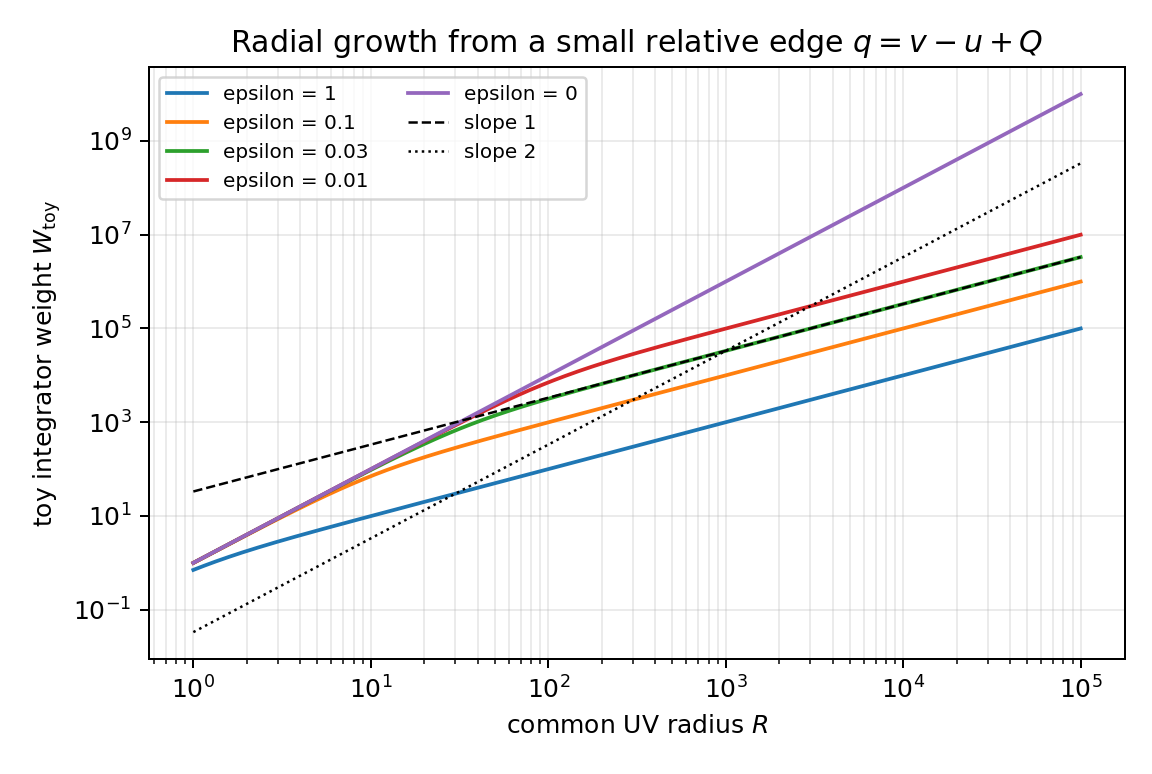
\includegraphics[width=0.78\textwidth]{figures/toy_radial_scaling.png}
  \caption{Toy-model radial scaling.  For fixed nonzero relative mismatch
  $\epsilon$, the weighted integrand approaches a slope-one growth,
  $W_{\rm toy}\sim R/\epsilon$.  Exact coalescence crosses over to slope two in
  this deliberately simplified model.}
  \label{fig:toy-radial}
\end{figure}

\begin{figure}[H]
  \centering
  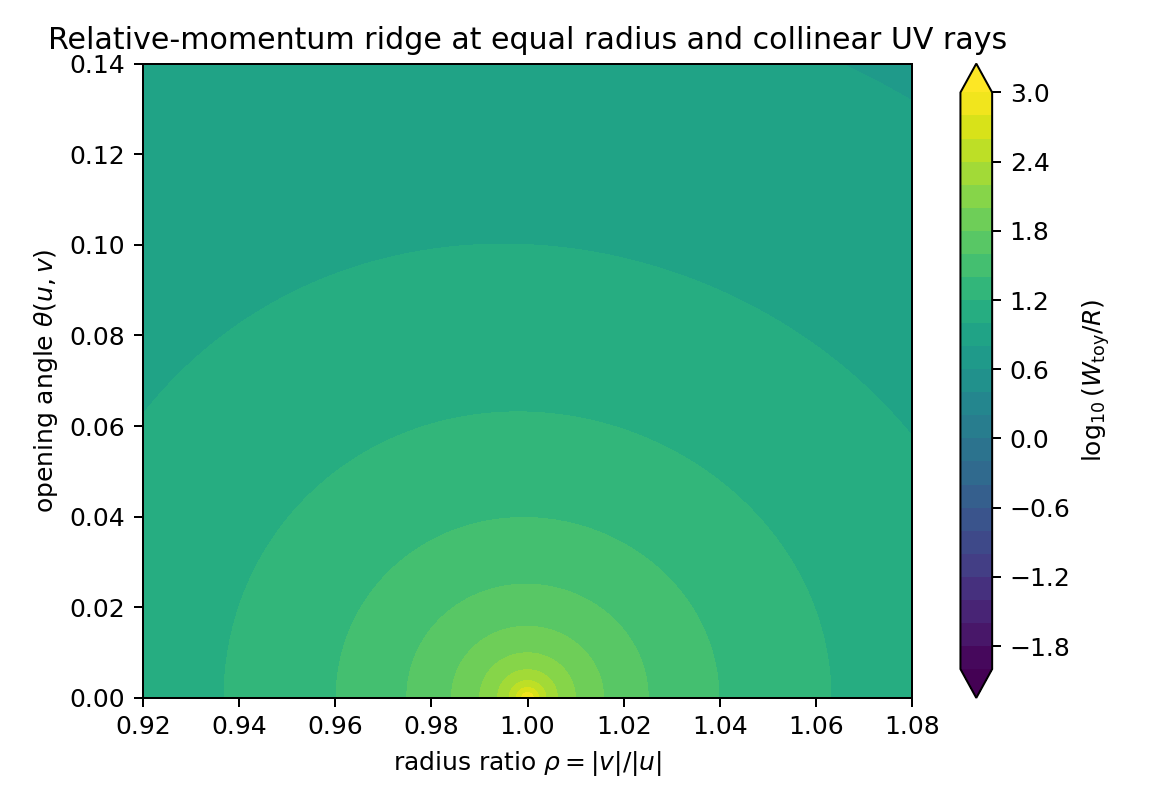
\includegraphics[width=0.78\textwidth]{figures/toy_relative_ridge.png}
  \caption{Toy relative-momentum ridge at fixed large common radius.  The
  enhancement is concentrated near equal radius, $\rho=1$, and small opening
  angle.  Existing LMB channels can reduce coefficients, but they do not create
  a direct sampling variable for this ridge.}
  \label{fig:toy-ridge}
\end{figure}

\section{GL00 approach data}

The GL00 radial scan starts from the high-weight point
\[
\begin{split}
  x_A = (&0.9938195811740000,\ 0.6303276140313304,\
          0.6037887485521857,\\
        &0.9939524818481166,\ 0.6277285639451646,\
          0.6151209153931045).
\end{split}
\]
At $\lambda=1$, the two radial variables correspond to approximately
\[
  r_0 \simeq 4.8240\times 10^4,\qquad
  r_1 \simeq 4.9307\times 10^4.
\]
The two radii are therefore both in the UV and within about two percent of each
other.  The angular coordinates are also close; the fitted opening angle in the
angular scan is
\[
  \theta_A \simeq 2.82\times 10^{-2}.
\]

The large-radius fit of the \GL{} inspected weight gives:
\begin{center}
\begin{tabular}{lccc}
\toprule
case & fit range & slope in $\log |W|$ vs. $\log\lambda$ & points\\
\midrule
LMB multichannel off & $\lambda\ge 1$ & 1.00005 & 27\\
LMB multichannel on  & $\lambda\ge 1$ & 1.00424 & 27\\
\bottomrule
\end{tabular}
\end{center}
The coefficient changes strongly when LMB multichanneling is enabled, but the
large-radius power does not.  This is the important observation: the current
multichanneling can reduce the normalization of the problematic ray, but it
does not alter the radial power seen by the integrator.

\begin{figure}[H]
  \centering
  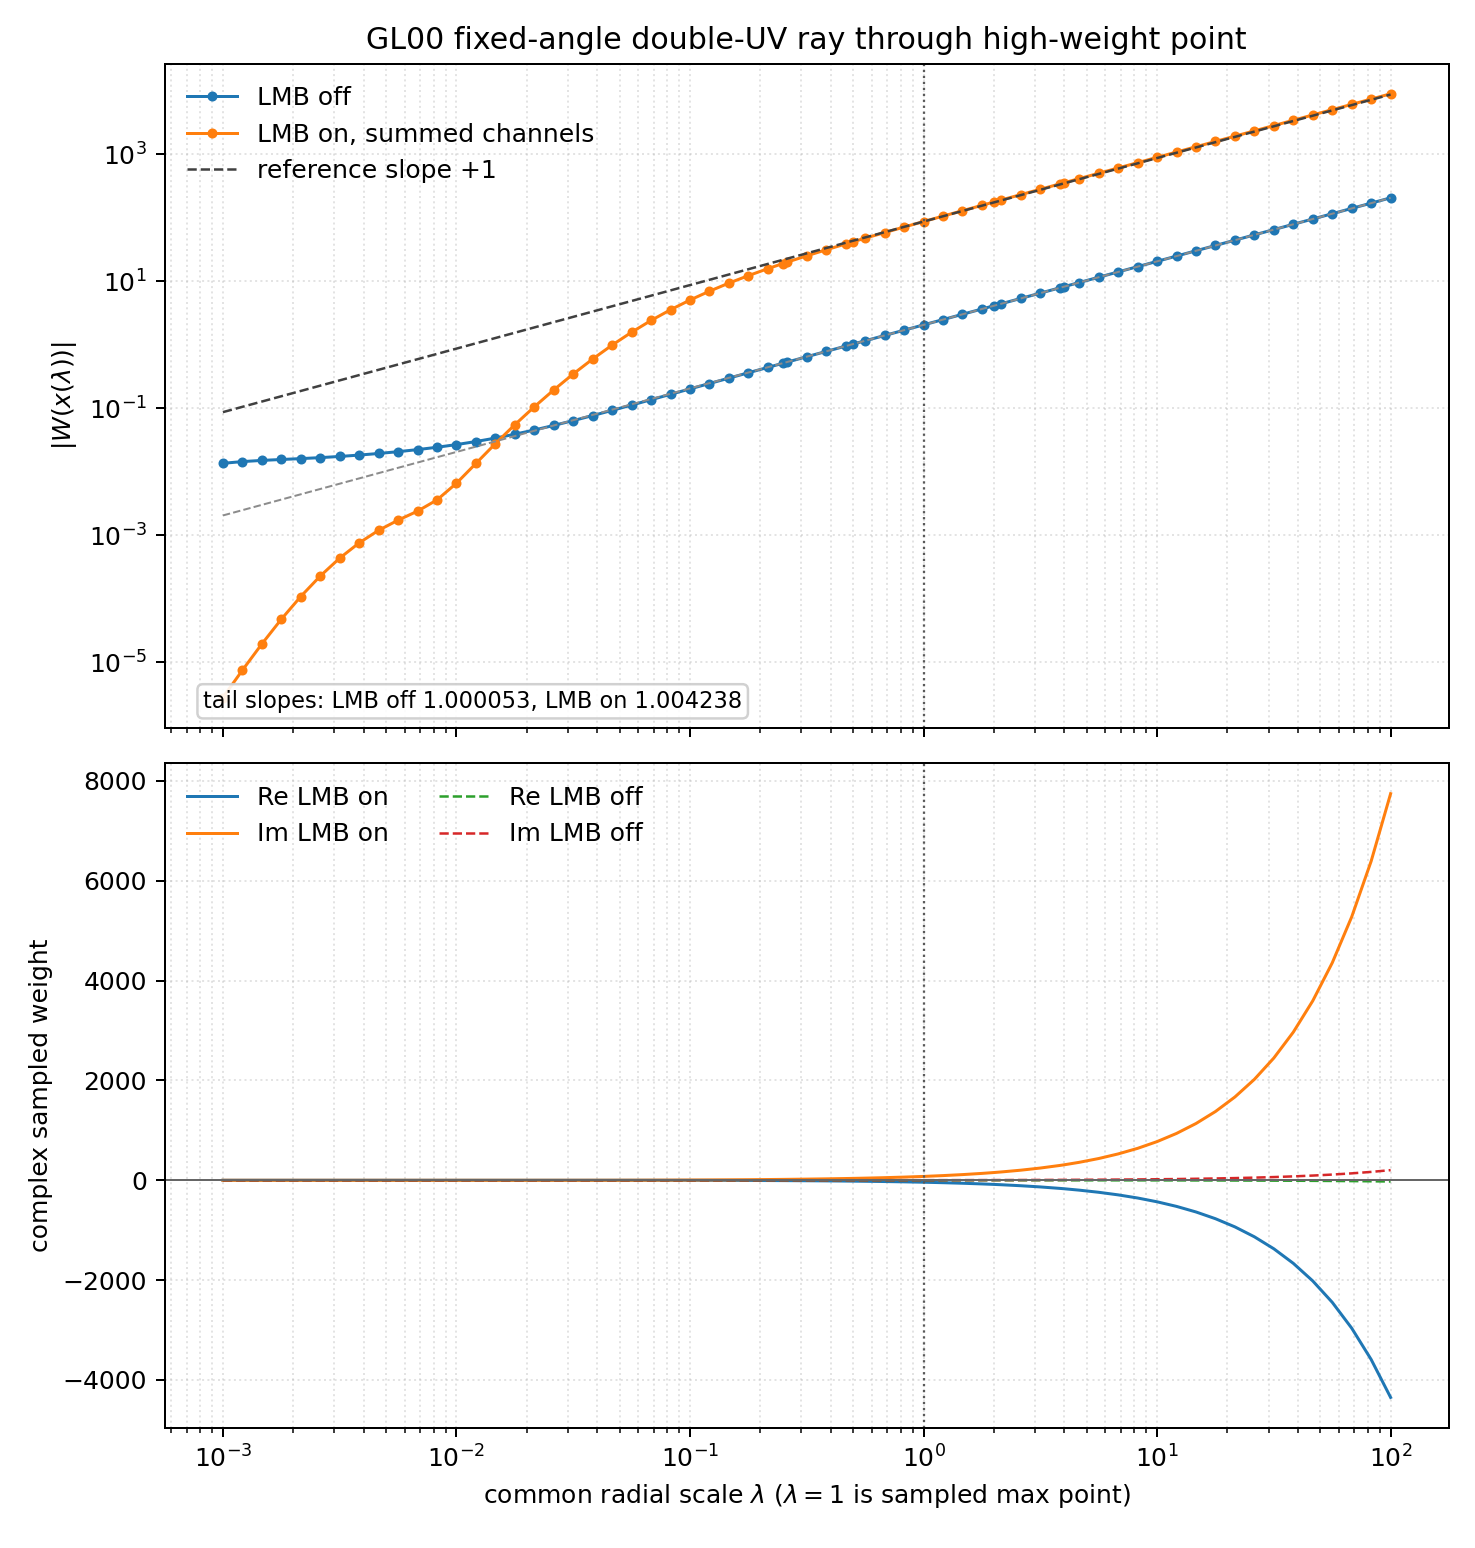
\includegraphics[width=0.78\textwidth]{figures/gl00_uv_ray_weight.png}
  \caption{\GL{} inspected event weight along the high-weight double-UV ray.
  All parameterization jacobians are included.  The large-radius behavior is
  approximately linear in the common UV scale.}
  \label{fig:gl00-ray}
\end{figure}

\begin{figure}[H]
  \centering
  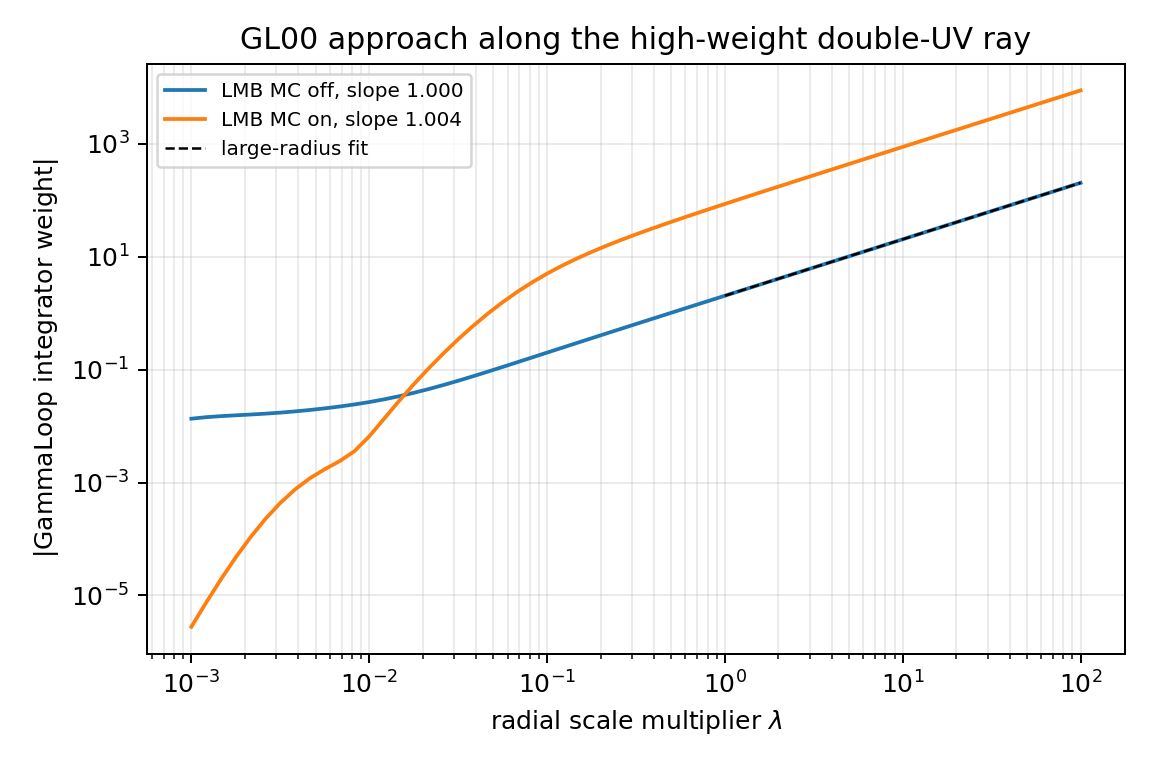
\includegraphics[width=0.78\textwidth]{figures/gl00_uv_ray_fit_compact.png}
  \caption{Compact replot of the same radial data, with large-radius fit
  slopes.  The fit is not intended to model the low-radius region.}
  \label{fig:gl00-ray-fit}
\end{figure}

\begin{figure}[H]
  \centering
  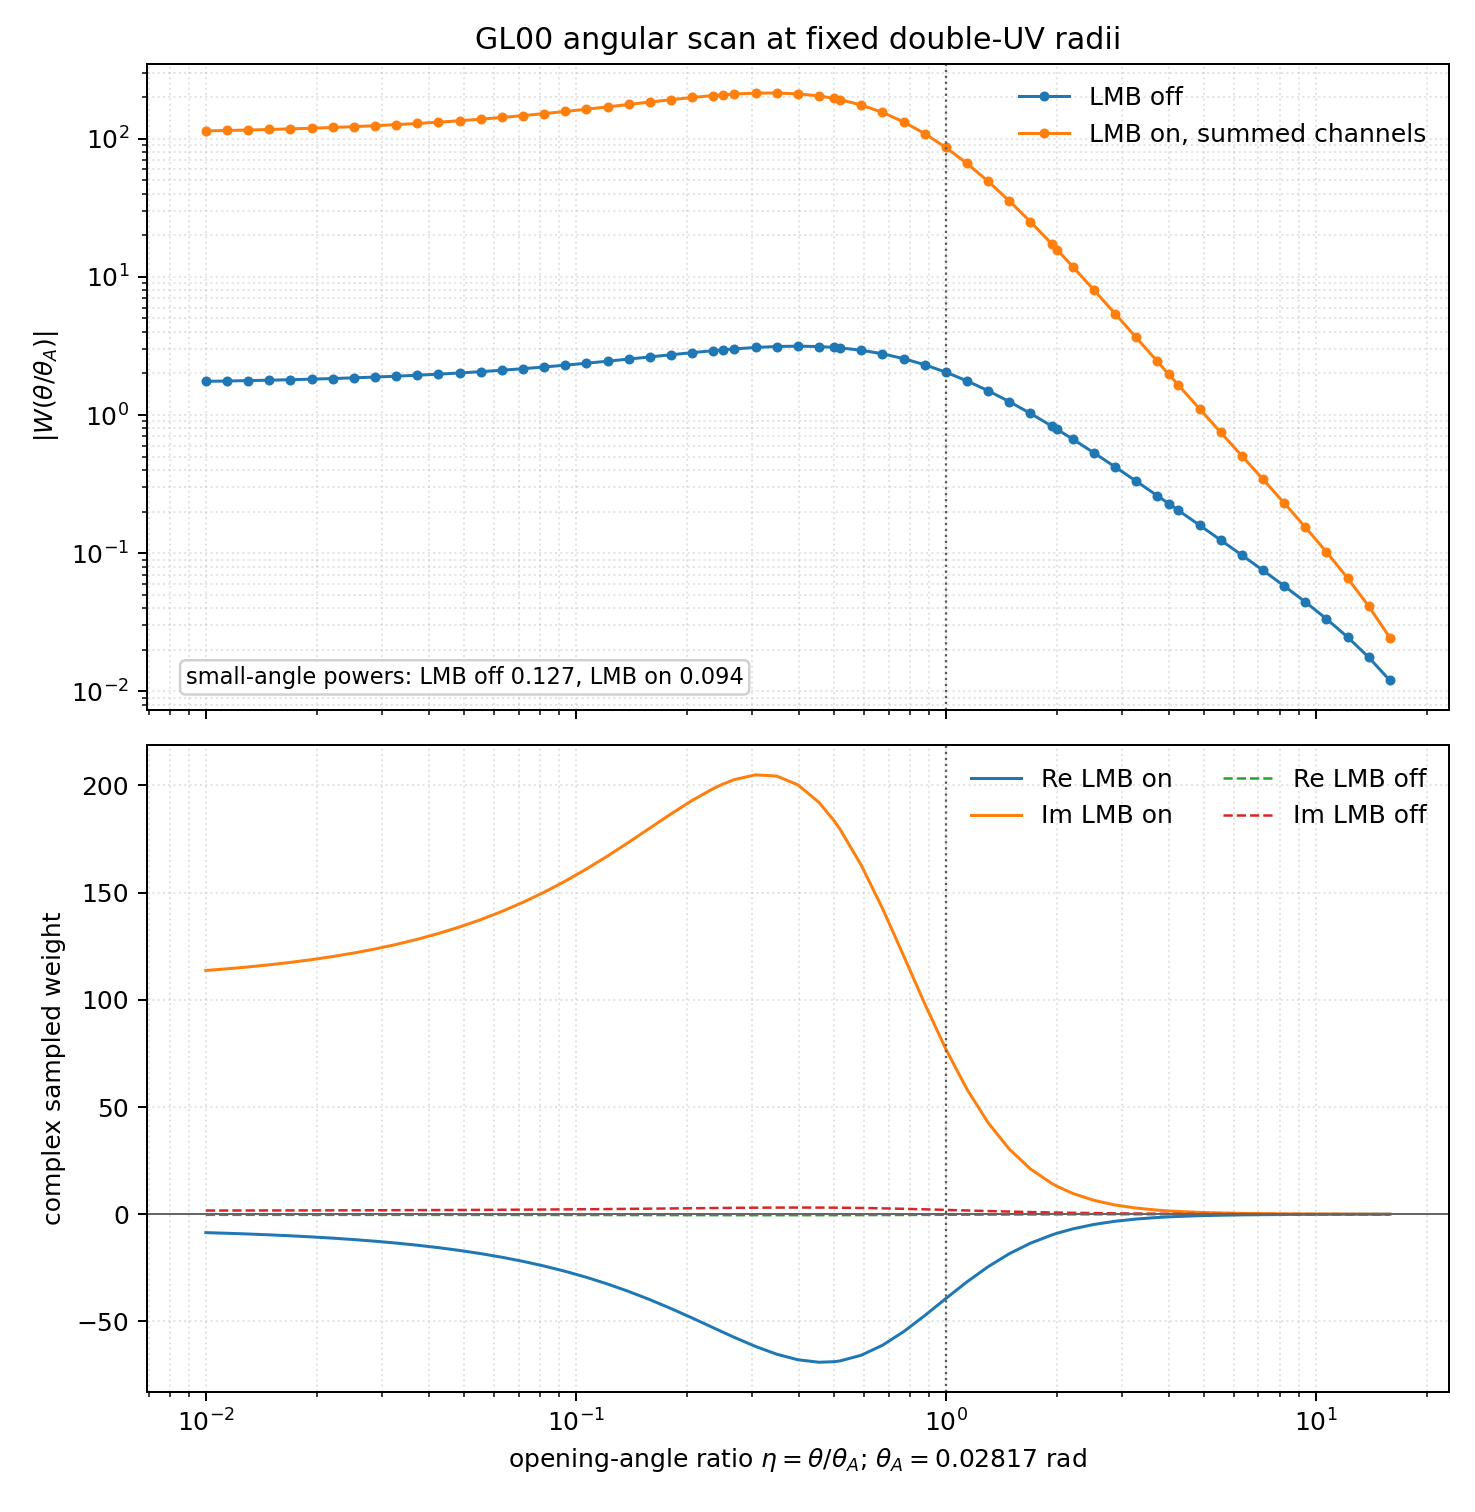
\includegraphics[width=0.78\textwidth]{figures/gl00_uv_angle_weight.png}
  \caption{Angular approach scan around the same GL00 point.  The coefficient
  is highly sensitive to the relative direction of the two hard rays, supporting
  the interpretation as a relative-momentum ridge rather than a generic
  double-UV failure.}
  \label{fig:gl00-angle}
\end{figure}

\section{Why the standard UV profile misses the enhancement}

The ordinary \texttt{profile ultra-violet} command samples one random
three-momentum per LMB loop variable and then rescales the selected subset.  It
therefore measures the generic large-momentum degree of divergence for that
sampled ray.  The relative-momentum ridge discussed above is a correlated
configuration: two UV rays must be nearly parallel and have nearly equal
radii, so that a physical edge momentum such as $v-u+Q$ stays anomalously
small compared to the two hard sampled basis momenta.  A random UV profile ray
hits this condition with probability zero.

There is also a conceptual difference between the UV profiler and the
integration-weight plots.  The profiler works directly in momentum space and
multiplies by the UV scaling measure factor used for the degree-of-divergence
test.  It does not include the full $x$-space parameterization jacobian,
adaptive discrete-channel probability, or the conformal-map density that define
the event weight seen by the integrator.  This is why the standard UV profile
can be clean while the integrator still sees a high-variance, locally
integrable ridge.

To make the correlated direction testable, the profiler now accepts fixed UV
ray data:
\begin{verbatim}
profile ultra-violet ... \
  --uv-ray-directions dx0 dy0 dz0 [dx1 dy1 dz1 ...] \
  --uv-ray-norms n0 [n1 ...]
\end{verbatim}
One direction or norm is repeated for all loop variables; otherwise one
three-vector and one norm can be supplied per loop variable.  If directions are
given but no norm is supplied, the default starting norm is $E_{\rm cm}$.

The same profiler was then run on the fixed ray matching the angular direction
and radius ratio of the GL00 approach scan:
\begin{verbatim}
--uv-ray-directions
  -0.66816740923660423 -0.71446756114601095 0.20757749710437134
  -0.67621171790860379 -0.69980455265688968 0.23024183078620908
--uv-ray-norms 1 1.0221114989619468
\end{verbatim}

The summed, not-per-orientation UV profiles are:
\begin{center}
\begin{tabular}{lccccc}
\toprule
profile & entries & worst slope & $r^2$ & bad entries & arb retry\\
\midrule
random ray, all subsets & 33 & $-0.997272$ & 0.999997 & 0/33 & 0/33\\
tailored ray, double-free subsets & 11 & $-0.812993$ & 0.986953 & 11/11 & 11/11\\
tailored ray, single-free subsets & 22 & $-1.000429$ & 1.000000 & 0/22 & 0/22\\
\bottomrule
\end{tabular}
\end{center}
Here ``bad'' means a fitted slope above the profiler warning threshold
$-0.9$.  The random-ray result is the expected generic UV profile.  With the
tailored ray, all double-free subsets move to the same fitted behavior,
\[
  \log |I_{\rm prof}| \simeq -0.812993 \log s + \mathrm{const},
  \qquad r^2=0.986953,
\]
and all of those double-free fits require the arbitrary-precision retry.
Single-free subsets remain ordinary.

A follow-up scan continuously shrinks the plot-ray mismatch.  Let $a=1$ denote
the GL00 plot ray above and $a=0$ denote the exactly collinear, equal-radius
ray with the first plot-ray direction used for both loop variables.  The second
direction is
\[
  \hat v(a)=\frac{(1-a)\hat u+a\hat v_{\rm plot}}
                  {\abs{(1-a)\hat u+a\hat v_{\rm plot}}},
  \qquad
  \rho(a)=1+a(\rho_{\rm plot}-1).
\]
The table reports the summed double-free UV-profile slope.  All 11 double-free
LMB subsets give the same number for each row.
\begin{center}
\small
\begin{tabular}{ccccc}
\toprule
$a$ & $\theta(\hat u,\hat v)$ & $\rho-1$ &
$10^3\!\to\!10^5$ & $10^3\!\to\!10^7$ \\
\midrule
1.000 & $2.817\times10^{-2}$ & $2.211\times10^{-2}$ & $-0.814$ & $-0.931$\\
0.500 & $1.408\times10^{-2}$ & $1.106\times10^{-2}$ & $-0.684$ & $-0.881$\\
0.200 & $5.633\times10^{-3}$ & $4.422\times10^{-3}$ & $-0.434$ & $-0.776$\\
0.100 & $2.817\times10^{-3}$ & $2.211\times10^{-3}$ & $-0.182$ & $-0.661$\\
0.050 & $1.408\times10^{-3}$ & $1.106\times10^{-3}$ & $+0.104$ & $-0.516$\\
0.020 & $5.633\times10^{-4}$ & $4.422\times10^{-4}$ & $+0.471$ & $-0.289$\\
0.010 & $2.816\times10^{-4}$ & $2.211\times10^{-4}$ & $+0.699$ & $-0.101$\\
0.005 & $1.408\times10^{-4}$ & $1.106\times10^{-4}$ & $+0.860$ & $+0.092$\\
0.000 & 0 & 0 & $+1.000$ & $+1.000$\\
\bottomrule
\end{tabular}
\end{center}
A sparse extension to $10^9$ gives slopes $-0.964$ for $a=1$, $-0.820$ for
$a=0.1$, $-0.611$ for $a=0.02$, $-0.376$ for $a=0.005$, and $+1.000$ for
$a=0$.  This is the expected non-uniform limit.  For any fixed nonzero
angular/radius mismatch, probing deep enough eventually resolves the relative
momentum and pushes the fit back toward the generic negative UV behavior.  As
the mismatch is reduced, the crossover moves to larger scales, and over the
finite UV windows relevant to the integrator the fitted slope degrades through
zero and becomes positive.  The exactly coincident GL00-direction ray remains
positive because the relative hard momentum is kept fixed to the external
shift instead of growing with the common UV scale.

The same two profiler runs were also repeated with \texttt{--per-orientation}.
For the random ray, the double-free per-orientation profile remained clean:
the worst double-free orientation slope was $-0.988527$, with no
arbitrary-precision retries and no slope above $-0.9$.  For the tailored ray,
the issue is not isolated to a unique orientation.  Among the 62 fitted
orientations, 48 have at least one double-free entry above $-0.9$.  The
strongest orientations are:
\begin{center}
\begin{tabular}{lcccc}
\toprule
orientation & max slope & avg. double-free slope & bad entries & arb retry\\
\midrule
\texttt{0000+++--++} & $-0.614883$ & $-0.614883$ & 11/11 & 11/11\\
\texttt{0000--+--+-} & $-0.615094$ & $-0.615094$ & 11/11 & 11/11\\
\texttt{0000+++--+-} & $-0.632973$ & $-0.632973$ & 11/11 & 11/11\\
\texttt{0000--+--++} & $-0.633049$ & $-0.633049$ & 11/11 & 11/11\\
\texttt{0000---++--} & $-0.709478$ & $-0.709478$ & 11/11 & 11/11\\
\texttt{0000++-++-+} & $-0.709620$ & $-0.709620$ & 11/11 & 11/11\\
\bottomrule
\end{tabular}
\end{center}
The repeated value across all 11 double-free LMB subsets is expected for this
fixed ray because the ray is supplied in each LMB basis.  Orientation
\texttt{0000+++--++} is the worst fitted one, but it is only slightly worse
than \texttt{0000--+--+-}; the enhancement is therefore a broad
orientation-sector feature rather than a single-orientation defect.

The z-axis exactly collinear equal-radius test ray, $(0,0,1)$ and $(0,0,1)$
with norms $1,1$, produced missing fits rather than stable slopes.  This was a
direction-specific numerical special case, not the generic behavior of
coincident rays; the GL00 plot-direction coincident ray gives the stable
positive slopes shown above.

These fixed-ray results are not evidence for a generic uncancelled UV
divergence.  They instead expose a non-uniform, codimension relative-momentum
ridge that the random-ray UV profile hides.

This is not in contradiction with the positive-slope event-weight plots.  The
UV profile uses momentum-space samples with \texttt{integrator\_weight=1} and
multiplies the raw integrand by only the scale-measure factor
$s^{3n_{\rm UV}}$.  For the double-UV tests here this is $s^6$.  The radial
approach plots, by contrast, show the density seen by the integrator after the
spherical linear map.  For one hard loop,
\[
  r = E_{\rm cm} b\,\frac{x}{1-x},
  \qquad
  r^2\frac{\dd r}{\dd x}\sim r^4 ,
\]
whereas the UV shell-measure factor used by the profiler is $r^3$ per loop.
Thus the plotted $x$-space weight contains one extra large-radius power per
hard loop compared to the profiler's DOD diagnostic.  A tailored-ray profiler
slope near $-0.813$ can therefore correspond to a pointwise $x$-space weight
that grows roughly like a positive power along the same radial approach.  When
the rays are tuned even closer together, the profiler itself finds zero or
positive slopes along that forced line.  The transverse angular and
radius-ratio volume is not represented by this one-dimensional profile, so the
positive forced-ray DOD identifies an integrable relative singularity and a
variance problem rather than a generic UV divergence of the full integral.

The profiler JSON and logs for the default, plot-ray, simplified split-ray,
exactly collinear, and per-orientation tests are saved in the report data
directory under the \texttt{uv\_profile\_*} filenames.

\section{Current long-run integration checks}

The current all-LMB one-million-sample diagnostic, using Monte Carlo over LMB
channels, kinematics A, helicity $+-+-$, $m_{\rm UV}=9.188$, and
$\mu_R=91.188$, gave:
\begin{center}
\begin{tabular}{lccc}
\toprule
component & value & error & relative error\\
\midrule
real & $-6.8192\times 10^{-6}$ & $4.7659\times 10^{-6}$ & 69.9\%\\
imag & $-5.4228\times 10^{-6}$ & $3.3372\times 10^{-6}$ & 61.5\%\\
\bottomrule
\end{tabular}
\end{center}
The largest signed weights in that run were:
\begin{center}
\begin{tabular}{lcc}
\toprule
component/sign & max evaluation & LMB channel\\
\midrule
real $+$ & $+5.3591\times 10^{-1}$ & $(5,9)$\\
real $-$ & $-4.3118$ & $(5,10)$\\
imag $+$ & $+5.4193\times 10^{-1}$ & $(5,9)$\\
imag $-$ & $-2.5294$ & $(5,10)$\\
\bottomrule
\end{tabular}
\end{center}

A longer Monte-Carlo-over-LMB run with $90\,\mathrm{M}$ samples and 20 cores
completed in $739.3\,\mathrm{s}$.  It did not reach the requested sub-10\%
Monte-Carlo error:
\begin{center}
\begin{tabular}{lcccc}
\toprule
component & value & error & relative error & max-weight impact\\
\midrule
real & $-4.4150\times 10^{-7}$ & $4.2964\times 10^{-7}$ & 97.3\% & 0.791\\
imag & $-1.2004\times 10^{-6}$ & $3.0318\times 10^{-7}$ & 25.3\% & 0.134\\
\bottomrule
\end{tabular}
\end{center}
The largest signed weights in this run moved to LMB channel $(5,7)$.  The
largest real negative event was $-31.4201$, and the largest imaginary negative
event was $-14.4356$, both at the same sampled point.  The adaptive grid
probability for channel $(5,7)$ was about 42.2\%, but the continuous relative
ridge still dominated the variance.

An explicit summed-LMB run with $10\,\mathrm{M}$ samples was run for a
comparable wall time, $740.9\,\mathrm{s}$.  Summing removes the discrete LMB
sampling noise but makes each sample roughly an order of magnitude more
expensive.  At equal wall time it also did not converge:
\begin{center}
\begin{tabular}{lcccc}
\toprule
component & value & error & relative error & max-weight impact\\
\midrule
real & $+6.6162\times 10^{-8}$ & $3.2102\times 10^{-7}$ & 485.2\% & 1.513\\
imag & $-1.1342\times 10^{-6}$ & $4.4162\times 10^{-7}$ & 38.9\% & 0.190\\
\bottomrule
\end{tabular}
\end{center}
The summed-channel run lowers the absolute largest sampled weights compared to
the MC-over-LMB run, but the real part is close enough to zero that its
relative error remains very large.  These results show that the default
$\alpha=3$ LMB multichannel setup did not reach stable sub-10\% errors in the
tested wall time.  They should not be read as proof that LMB multichanneling is
irrelevant, or that no choice of $\alpha$ can help; the unresolved issue is the
continuous relative-momentum ridge left after the discrete OSE reweighting.

The saved run artifacts are in the report data directory, with separate JSON
and log files for the \(90\,\mathrm{M}\) MC-over-LMB run and the \(10\,\mathrm{M}\)
summed-LMB run.

\section{What the LMB multichannel prefactor does}

The generated all-LMB setup contains channels where edge 4 is a basis edge, and
the LMB multichanneling code does use this information.  For a channel $c$ with
basis edges $e\in c$, the channel weight is
\begin{equation}
  w_c=\left(\prod_{e\in c} E_e\right)^{-\alpha},
  \qquad
  p_c=\frac{w_c}{\sum_j w_j}.
  \label{eq:lmb-channel-weight}
\end{equation}
With \texttt{lmb\_channels = "monte\_carlo"}, one LMB is sampled with this
normalized weight.  With \texttt{lmb\_channels = "summed"}, all generated LMBs
are evaluated with the same normalized prefactors.  The default value is
$\alpha=3$, and the flat \texttt{[sampling]} parser now exposes this as an
\texttt{alpha} field so that it can be scanned directly.

I evaluated this normalized prefactor on the same ray family used in the
fixed-ray UV-profile scan.  The table reports the raw probability assigned to
the problematic $(5,10)$ interpretation and the total probability assigned to
channels containing edge 4:
\begin{center}
\small
\begin{tabular}{cccccc}
\toprule
$a$ & $R$ & $\alpha$ & $E_4/R$ & $p_{(5,10)}$ & $\sum_{4\in c}p_c$\\
\midrule
1.000 & $10^3$ & 1 & $2.041\times10^{-1}$ & $3.050\times10^{-2}$ & 0.854066\\
1.000 & $10^3$ & 3 & $2.041\times10^{-1}$ & $1.621\times10^{-3}$ & 0.992885\\
1.000 & $10^7$ & 1 & $3.566\times10^{-2}$ & $5.814\times10^{-3}$ & 0.970933\\
1.000 & $10^7$ & 3 & $3.566\times10^{-2}$ & $7.726\times10^{-6}$ & 0.999961\\
0.100 & $10^7$ & 1 & $3.584\times10^{-3}$ & $5.959\times10^{-4}$ & 0.997020\\
0.100 & $10^7$ & 3 & $3.584\times10^{-3}$ & $7.687\times10^{-9}$ & 1.000000\\
0.020 & $10^7$ & 1 & $7.206\times10^{-4}$ & $1.200\times10^{-4}$ & 0.999400\\
0.020 & $10^7$ & 3 & $7.206\times10^{-4}$ & $6.240\times10^{-11}$ & 1.000000\\
0.005 & $10^7$ & 1 & $1.843\times10^{-4}$ & $3.072\times10^{-5}$ & 0.999846\\
0.005 & $10^7$ & 3 & $1.843\times10^{-4}$ & $1.044\times10^{-12}$ & 1.000000\\
0.000 & $10^7$ & 1 & $1.973\times10^{-5}$ & $3.287\times10^{-6}$ & 0.999984\\
0.000 & $10^7$ & 3 & $1.973\times10^{-5}$ & $1.279\times10^{-15}$ & 1.000000\\
\bottomrule
\end{tabular}
\end{center}
The conclusion is that the OSE prefactor is doing something very strong.  On
the near-collinear rays, default $\alpha=3$ assigns essentially all normalized
channel weight to LMBs containing edge 4 and suppresses the direct $(5,10)$
interpretation by many orders of magnitude.  Increasing $\alpha$ would make
this channel selection even sharper; decreasing it would make the channel
selection smoother.  Therefore the previous statement that LMB MC merely
samples an LMB, or that it cannot be sufficient by construction, would be too
strong.

What remains true is that this prefactor is a discrete LMB reweighting, not a
continuous change of variables to
\[
  P_{\rm common}\simeq \frac{u+v}{2},
  \qquad
  q = v-u+Q.
\]
The problematic region is thin in the original hard-momentum variables and
natural in $(P_{\rm common},q)$ variables.  Once the mismatch is fixed and all
relevant OSEs scale linearly with the common hard radius, changing $\alpha$
changes the coefficient and channel allocation but not the asymptotic radial
power along that ray.  Near the exact edge-small limit it can be decisive,
because $E_4/R$ becomes tiny and the normalized weight overwhelmingly selects
edge-4 channels.

This explains why the longer all-LMB Monte-Carlo run assigned large
probability to channel $(5,7)$, about 42.2\%, and sizable probabilities to
channels such as $(5,10)$, about 15.8\%, while individual edge-4 channels were
only about 1.4\% each.  The adaptive procedure sees the contribution and
variance of the existing channels, but it does not infer a new
relative-momentum map.  The current data are therefore compatible with two
possibilities: default $\alpha=3$ may simply need more statistics or tuning, or
the variance may require an explicit relative-momentum channel in addition to
the OSE-prefactor LMB selection.  An $\alpha$ scan should be part of the next
integration campaign now that the setting is exposed in \texttt{[sampling]}.

\section{Other \texorpdfstring{$\gamma\gamma\to\gamma\gamma$}{aa to aa} two-loop graphs}

I also ran the same integrated-UV generation and profiling campaign on the
other \texttt{aa\_aa} two-loop graph labels selected by the feyngen card:
\texttt{GL01}, \texttt{GL03}, \texttt{GL05}, \texttt{GL06}, \texttt{GL08},
\texttt{GL12}, \texttt{GL14}, \texttt{GL16}, \texttt{GL17}, and
\texttt{GL18}.  The command line was protected with a 100 GiB virtual-memory
limit.  For every profiling and integration attempt I used kinematics A,
helicity $+-+-$, disabled thresholds, $\mu_R=91.188$, and $m_{\rm UV}=9.188$.
For the graphs that generated successfully, the integration run used 20 cores,
$90\,\mathrm{M}$ samples, summed orientations, generated LMB multichanneling
with summed LMB channels, and the exposed default $\alpha=3$ OSE prefactor.

Seven of the ten non-GL00 labels failed before a UV profile could be produced.
The feyngen step did select and write a single diagram, but the following
\texttt{generate existing} step failed during integrated-UV processing at
\texttt{crates/gammalooprs/src/uv/approx/integrated.rs:279}, inside the vakint
tensor-reduction path, with \texttt{No such file or directory (os error 2)}.
These were fast failures, not memory blow-ups under the 100 GiB cap.

\begin{center}
\scriptsize
\begin{tabular}{p{0.06\linewidth}p{0.25\linewidth}p{0.22\linewidth}p{0.29\linewidth}}
\toprule
graph & generation & UV profile & integration and convergence\\
\midrule
\texttt{GL01} &
feyngen 16 s; generation/profile wall 18.0 s; integrated-UV tensor reduction failed &
not available &
not run\\
\texttt{GL03} &
feyngen 8 s; generation/profile wall 10.2 s; integrated-UV tensor reduction failed &
not available &
not run\\
\texttt{GL05} &
feyngen 24 s; generation/profile wall 27.4 s; integrated-UV tensor reduction failed &
not available &
not run\\
\texttt{GL06} &
feyngen 7 s; generation/profile wall 10.5 s; integrated-UV tensor reduction failed &
not available &
not run\\
\texttt{GL08} &
feyngen 29 s; integrand generation row: expr 2.97 s, spenso 0.136 s, Symbolica eval 7.62 s; generation+profile wall 44.2 s; peak RAM 2.26 GiB &
45 entries; worst slope $-0.99796$; no slopes above $-0.9$; no arb retries &
avg total/integrand runtime 60.6/28.4 $\mu$s per sample per core; real
$6.3157(2.4546)\times10^{-7}$, 38.9\%; imag
$-9.5480(1.8487)\times10^{-7}$, 19.4\%; not converged\\
\texttt{GL12} &
feyngen 11 s; integrand generation row: expr 2.99 s, spenso 0.176 s, Symbolica eval 6.83 s; generation+profile wall 25.0 s; peak RAM 1.90 GiB &
45 entries; worst slope $-0.99545$; no slopes above $-0.9$; no arb retries &
avg total/integrand runtime 61.1/28.7 $\mu$s per sample per core; real
$8.8850(19.2521)\times10^{-8}$, 216.7\%; imag
$6.1223(1.5717)\times10^{-7}$, 25.7\%; not converged\\
\texttt{GL14} &
feyngen 2 s; generation/profile wall 5.9 s; integrated-UV tensor reduction failed &
not available &
not run\\
\texttt{GL16} &
feyngen 27 s; integrand generation row: expr 2.91 s, spenso 0.137 s, Symbolica eval 7.83 s; generation+profile wall 42.1 s; peak RAM 2.16 GiB &
45 entries; worst slope $-0.99940$; no slopes above $-0.9$; no arb retries &
avg total/integrand runtime 61.4/28.7 $\mu$s per sample per core; real
$1.4087(2.1772)\times10^{-7}$, 154.6\%; imag
$-3.6861(0.3847)\times10^{-6}$, 10.4\%; imaginary part nearly converged,
but the graph is not converged overall\\
\texttt{GL17} &
feyngen 10 s; generation/profile wall 12.4 s; integrated-UV tensor reduction failed &
not available &
not run\\
\texttt{GL18} &
feyngen 6 s; generation/profile wall 9.9 s; integrated-UV tensor reduction failed &
not available &
not run\\
\bottomrule
\end{tabular}
\end{center}

The three graphs that passed integrated-UV generation, \texttt{GL08},
\texttt{GL12}, and \texttt{GL16}, all have clean random-ray UV profiles:
their worst fitted slopes stay below $-0.995$, all fitted DODs are negative,
and none required arbitrary-precision rescue.  At $90\,\mathrm{M}$ samples the
per-sample timing is also stable, about $60$--$61\,\mu$s total and
$28$--$29\,\mu$s in the integrand itself per core.  Nevertheless none of these
three reached sub-10\% Monte-Carlo error in both the real and imaginary parts.
\texttt{GL16} is closest, with a 10.4\% imaginary-part relative error, but its
real part is still compatible with zero at the present statistics.  The
successful graphs therefore do not show the GL00 catastrophic double-UV ridge
in the same way, but they are not yet precision-converged diagram-level
integrals in this setup.

The compact campaign summary, per-graph generation logs, successful UV-profile
JSON files, and successful \(90\,\mathrm{M}\)-sample integration logs/results
are archived in the report data directory under
\texttt{aa\_aa\_2l\_graph\_campaign}.

\section{Implications}

The current evidence points to a high-variance, locally integrable
relative-momentum singularity rather than a wrong integrated UV counterterm or a
missing local UV cancellation.  The practical options suggested by the toy
model are:
\begin{enumerate}
  \item add a specialized channel or remapping for hard-hard relative momentum
        ridges, using variables close to $(P_{\rm common},q)$;
  \item scan the LMB prefactor exponent $\alpha$; larger values focus more
        strongly on channels containing the small OSE, while smaller values
        avoid over-focusing and may improve other regions;
  \item use explicit summed LMB channels as a diagnostic, while recognizing
        that this reduces discrete-channel variance but does not by itself
        remap the continuous relative-ridge variables.
\end{enumerate}

\end{document}
